\lcTex{%
  \newlength{\widthExtra}\setlength{\widthExtra}{1.1cm}
  \newlength{\widthLineReal}\setlength{\widthLineReal}{\linewidth}
  \addtolength{\widthLineReal}{-\widthExtra}
  \newlength{\minipageSpace}\setlength{\minipageSpace}{0.2cm}

  \newlength{\widthLeft}
  \newlength{\widthRight}
}

\newcommand{\reals}{{\rm I\!\hspace{-0.025em} R}}
\newcommand{\calC}{{\cal C}}
\newcommand{\calA}{{\cal A}}
\newcommand{\eps}{{\varepsilon}}
\newcommand{\dcel}{{\sc Dcel}}
\newcommand{\naive}{na\"{\i}ve}
\newcommand{\kdtree}{{\sc Kd}-tree}

% ===============================================================
\section{Introduction}
\label{bobs_sec:intro}
% ===============================================================
%
\begin{figure}[!htp]
\begin{ccTexOnly}
\begin{center}
\begin{tabular}{cccc}
  \pspicture[](-1,-2.3)(1,2)
    \psset{unit=1cm,linewidth=1pt}
    \pscircle*[linecolor=gray](0,-1){1}
    \pscircle*[linecolor=gray](0,1){1}
    \pscircle(0,-1){1}
    \pscircle(0,1){1}
    \psline{->}(0,0)(0,1)
    \psline{->}(0,0)(1,0)
  \endpspicture &
  \pspicture[](-2,-2.3)(2,2)
    \psset{unit=1cm,linewidth=1pt}
    \pscircle*[linecolor=gray](-1,0){1}
    \pscircle*[linecolor=gray](1,0){1}
    \pscircle(-1,0){1}
    \pscircle(1,0){1}
    \psline{->}(0,0)(0,1)
    \psline{->}(0,0)(1,0)
  \endpspicture &
  \pspicture[](-2,-2.3)(2,2)
    \psset{unit=1cm,linewidth=1pt}
    \pscustom[linewidth=0,fillstyle=solid,fillcolor=gray]{
      \psarc(0,1){1}{270}{360}
      \psarc(1,0){1}{90}{180}
    }
    \pscustom[linewidth=0,fillstyle=solid,fillcolor=gray]{
      \psarc(1,0){1}{180}{270}
      \psarc(0,-1){1}{0}{90}
    }
    \pscustom[linewidth=0,fillstyle=solid,fillcolor=gray]{
      \psarc(0,-1){1}{90}{180}
      \psarc(-1,0){1}{270}{360}
    }
    \pscustom[linewidth=0,fillstyle=solid,fillcolor=gray]{
      \psarc(-1,0){1}{0}{90}
      \psarc(0,1){1}{180}{270}
    }
    \psarc(0,1){1}{270}{360}
    \psarc{c}(1,0){1}{90}{180}
    \psarc(1,0){1}{180}{270}
    \psarc{c}(0,-1){1}{0}{90}
    \psarc(0,-1){1}{90}{180}
    \psarc{c}(-1,0){1}{270}{360}
    \psarc{-c}(-1,0){1}{0}{90}
    \psarc(0,1){1}{180}{270}
  \endpspicture &
  \pspicture[](-2,-2.3)(2,2)
    \psset{unit=1cm,linewidth=1pt}
    \pscustom[linewidth=0,fillstyle=solid,fillcolor=gray,linecolor=gray]{
      \psarc(0,1){1}{360}{180}
      \psarc(1,0){1}{90}{180}
      \psarc(-1,0){1}{0}{90}
    }
    \pscustom[linewidth=0,fillstyle=solid,fillcolor=gray,linecolor=gray]{
      \psarc(1,0){1}{270}{90}
      \psarc(0,-1){1}{0}{90}
      \psarc(0,1){1}{270}{0}
    }
    \pscustom[linewidth=0,fillstyle=solid,fillcolor=gray,linecolor=gray]{
      \psarc(0,-1){1}{180}{0}
      \psarc(-1,0){1}{270}{360}
      \psarc(1,0){1}{180}{270}
    }
    \pscustom[linewidth=0,fillstyle=solid,fillcolor=gray,linecolor=gray]{
      \psarc(-1,0){1}{90}{270}
      \psarc(0,1){1}{180}{270}
      \psarc(0,-1){1}{90}{180}
    }
    \pscircle(0,-1){1}
    \pscircle(0,1){1}
    \pscircle(-1,0){1}
    \pscircle(1,0){1}
  \endpspicture\\
  & & intersection & symmetric difference
\end{tabular}
\end{center}

\end{ccTexOnly}
\begin{ccHtmlOnly}
  <p><center>
    <img src="./fig/teaser.gif" border=0 alt="Boolean Set Operations">
  </center>
\end{ccHtmlOnly}
\caption{Examples of Boolean Set Operations.} 
\label{fig:teaser}
\end{figure}

This package consists of the implementation of Boolean set-operations
on point sets bounded by $x$-monotone curves in 2-dimensional
Euclidean space. In particular, it contains the implementation of
{\em regularized} Boolean set-operations, intersection predicates, and
point containment predicates. Figure~\ref{fig:teaser} shows simple examples 
of such operations.
% and Minkowski sum computations.

\begin{ccHtmlOnly}<p>\end{ccHtmlOnly}
A regularized Boolean set-operation $\mbox{op}^*$ can be obtained by
first taking the interior of the resultant point set of an {\em ordinary}
Boolean set-operation $(P\ \mbox{op}\ Q)$ and then by taking the
closure~\cite{cgal:h-sm-04}. That is
$P\ \mbox{op}^*\ Q = \mbox{closure}(\mbox{interior} (P\ \mbox{op}\ Q))$.
Regularized Boolean set-operations appear in Constructive Solid
Geometry (CSG), because regular sets are closed under regularized
Boolean set-operations, and because regularization eliminates lower
dimensional features, thus simplifying and restricting the
representation to physically meaningful solids.
% A simplified representation does not have to store selection marks;
% they are implicitly always set for vertices and edges, and for faces
% they are deduced from a suitably chosen orientation condition on their
% boundaries.
Ordinary Boolean set-operations, which distinguish between the
interior and the boundary of a polygon, are not implemented yet. These
operations operate on, and result with, general polygons, which
include isolated curves and points, and open shapes. The \ccc{Nef_2}
package supports these operation for (linear) polygons; see
Chapter~\ref{chap:nef_2}. 
% Bounding box constructions, extreme vertex provision, and point containment 
% predicates on a single (linear) polygon are provided by the 
% \ccc{Polygon_2} class; see Chapter~\ref{Polygon}.

\newpage
\lcTex{%
  \setlength{\widthRight}{4cm}
  \setlength{\widthLeft}{\widthLineReal}
  \addtolength{\widthLeft}{-\widthRight}
  \begin{minipage}{\widthLeft}
}
\label{fig:non_strictly_simple_polygon}
\begin{ccHtmlOnly}
  <p><center>
    <img src="./fig/fig_non_strictly_simple.gif" border=0 alt="A non strictly simple polygon" align=right>
  </center>
\end{ccHtmlOnly}
A polygon $P$ is said to be {\em simple} (or Jordan) if the
only points of the plane belonging to two polygon edges of $P$ are the
polygon vertices of $P$. Such a polygon has a well-defined interior
and exterior. Simple polygons are topologically equivalent to
a disk. A polygon in our context must be simple. The cyclic
sequence of alternating polygon edges and polygon vertices is referred
to as the polygon {\em boundary}. A polygon whose boundary contains the
same vertex twice or more is connected and simple but not
necessary strictly simple; see Figure~\ref{fig:non_strictly_simple_polygon}. 
We extend the notion of a polygon to a point set in $\mathrm{E}^2$ that has 
a topology of a polygon and its boundary edges must map to $x$-monotone
curves, and refer to it as a {\em general polygon}. We sometimes use
the term {\em polygon} instead of general polygon for simplicity hereafter.
\lcTex{%
  \end{minipage}\hspace{\minipageSpace}
  \begin{minipage}{\widthRight}
    \begin{center}
    
\includegraphics{Boolean_set_operations_2/fig/non_strictly_simple}
    \end{center}
    A non strictly simple polygon.
  \end{minipage}
}

% ===============================================================
\section{Boolean Set-Operations on General Polygons}
\label{bobs_sec:bops}
% ===============================================================
For two point sets $P$ and $Q$, the ordinary Boolean set-operations are
defined as follows:
\begin{description}
\item [Intersection predicate] tests whether the two polygons $P$ and $Q$
  overlap without explicitly computing the overlapping polygon if exists.
\item[Intersection] computes the intersection $R = P \cap Q$.
\item[Join] computes the union $R = P \cup Q$.
\item [Difference] computes the difference $R = P \setminus Q$ 
\item [Symmetric Difference] computes the symmetric difference
  $P = (P \setminus Q) \cup (Q \setminus P)$
\item[Complement] computes the complement
\lcTex{$R = \overline{P}$}
\lcRawHtml{<i>R = <span style="text-decoration: overline;">P</span></i>}
\end{description}

% ===============================================================
% \subsection{Regularized Boolean-Set Operations on General Polygons}
% \laabel{bso_ssec:regularized_bops}
% ===============================================================
A general polygon, which is an operand or a result of a regularized
Boolean set-operation is considered as being a closed point-set (that
consist of its interior and its boundary). The distinction between the 
interior and  the exterior of a polygon that results from a regularized 
Boolean set-operation is determined by the order of its vertices. 
The definition of the regularized Boolean set-operations 
is slightly different from the definition of the ordinary set operations
given above. For example, the intersection predicate tests whether the 
interior of two polygons $P$ and $Q$ overlap. Thus, if two polygons have 
a finite set of points, or even a boundary curve, in common, they are 
considered non-intersecting.

% ===============================================================
\section{The Main Components}
\label{bobs_sec:main_components}
% ===============================================================
The central component in the Boolean Set-Operations package is the
\ccc{General_polygon_set_2} class-template. It employs the
\ccc{Arrangement_2} class to represent a point set in the plane as a
planar arrangement; see Chapter~\ref{chapterArrangement_2}. 
An instance of the \ccc{General_polygon_set_2} class-template can be
constructed from general polygons or general polygons with holes. The
precise definitions of these polygons are provided in the following
subsections. The class template provides methods to apply regularized 
Boolean set-operations on pairs of instances of \ccc{General_polygon_set_2} 
or general polygon (or general polygon with holes) directly, and a few
other utility methods, with the method to compute the complement being 
an exception, as it accepts a single instance of one of the types above. 
The input and output of these methods consist of one or more general 
polygons, some of which may have holes.

\begin{ccHtmlOnly}<p>\end{ccHtmlOnly}
The package also contains free functions that perform common operations,
and are provided for convenience. A typical such function constructs a pair
of \ccc{General_polygon_set_2} instances, invokes the appropriate method to
apply the desired Boolean operation, and results with a Boolean value, or at
least one general polygon. When several operations are performed in a 
sequence, it is much more efficient to use the member functions of the
\ccc{General_polygon_set_2} type directly, as the extraction of the general
polygons from the internal representation for some operation, and the
reconstruction of the internal representation for the succeeding operation
could be time consuming.

% ---------------------------------------------------------------
\subsection{A Simple Example}
\label{bso_ssec:simple_example}
% ---------------------------------------------------------------
\lcTex{%
  \setlength{\widthRight}{2cm}
  \setlength{\widthLeft}{\widthLineReal}
  \addtolength{\widthLeft}{-\widthRight}
  \begin{minipage}{\widthLeft}
}
\label{fig:example}
\begin{ccHtmlOnly}
  <p><center>
    <img src="./fig/fig_triangles.gif" border=0 alt="Two triangles" align=right>
  </center>
\end{ccHtmlOnly}
Testing whether two polygons intersect results with a Boolean value, 
and does not require any additional data beyond the provision of the 
two polygons. The example listed below tests whether the two triangles 
depicted on the right intersect.
\lcTex{%
  \end{minipage}\hspace{\minipageSpace}
  \begin{minipage}{\widthRight}
    \begin{center}
    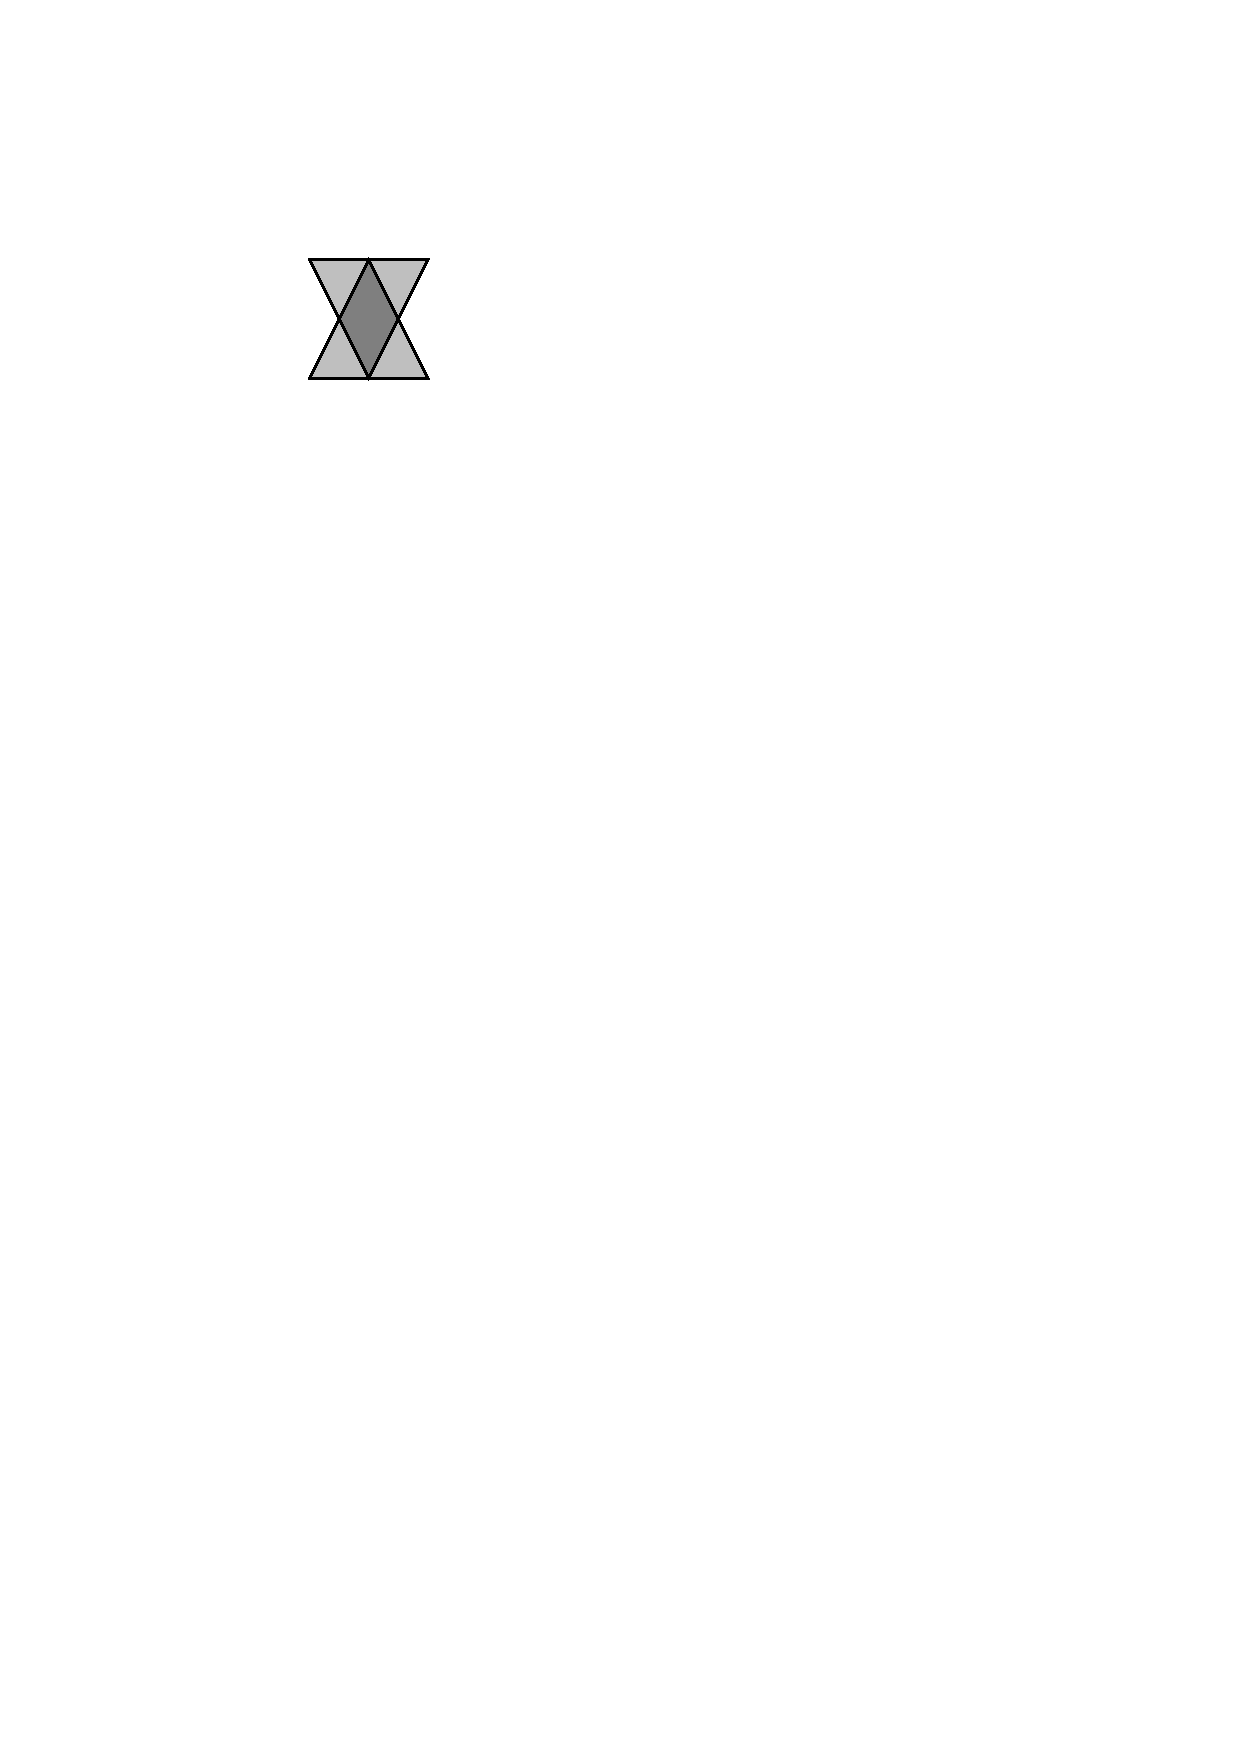
\includegraphics{Boolean_set_operations_2/fig/triangles}
    \end{center}
  \end{minipage}
}

\ccIncludeExampleCode{../examples/Boolean_set_operations_2/ex_do_intersect.C}

% ---------------------------------------------------------------
\subsection{Free Functions}
\label{bso_ssec:free_functions}
% ---------------------------------------------------------------
In many cases a simple operation that operates on two strictly simple
polygons that have no holes are required. The most simple functions in
the package operate on two polygons and accept them as two separate
parameters. However, even a simple operation, such as the union of two
strictly simple polygons with no holes, may result with a polygon with
holes, see Figure~\ref{fig:simple}~(a). Moreover, a simple operation,
such as the intersection of two strictly simple polygons with no holes, 
may result with a set of disjoint polygons; see
Figure~\ref{fig:simple}~(b). Finally, only a polygon with holes can
represent the complement of a polygon without holes. Notice that this
polygon has no outer boundary; see Figure~\ref{fig:simple}~(c).

\begin{figure}[!htp]
\begin{ccTexOnly}
\begin{center}
\begin{tabular}{ccc}
\pspicture[](0,0)(3,2)
\psset{unit=1cm,linewidth=1pt}
  \pspolygon*[linecolor=gray](0,1)(2,0)(1,1)(2,2)
  \pspolygon*[linecolor=gray](3,1)(1,2)(2,1)(1,0)
  \pspolygon(0,1)(2,0)(1,1)(2,2)
  \pspolygon(3,1)(1,2)(2,1)(1,0)
\endpspicture &
\pspicture[](0,0)(5,2)
\psset{unit=1cm,linewidth=1pt}
  \pspolygon*[linecolor=lightgray](0,0)(1.5,1.5)(2.5,0.5)(3.5,1.5)(5,0)
  \pspolygon*[linecolor=lightgray](0,2)(5,2)(3.5,0.5)(2.5,1.5)(1.5,0.5)
  \pspolygon*[linecolor=gray](1,1)(1.5,1.5)(2,1)(1.5,0.5)
  \pspolygon*[linecolor=gray](3,1)(3.5,1.5)(4,1)(3.5,0.5)
  \pspolygon(0,0)(1.5,1.5)(2.5,0.5)(3.5,1.5)(5,0)
  \pspolygon(0,2)(5,2)(3.5,0.5)(2.5,1.5)(1.5,0.5)
\endpspicture &
\pspicture[](0,0)(3,2)
\psset{unit=1cm,linewidth=1pt}
  \pspolygon*[linecolor=gray](0,2)(0,0)(3,0)(3,2)
  \pspolygon*[linecolor=lightgray](1,0.67)(2,0.67)(2,1.34)(1,1.34)
  \pspolygon[linecolor=black](1,0.67)(2,0.67)(2,1.34)(1,1.34)
\endpspicture
\\
(a) & (b) & (c)
\end{tabular}
\end{center}

\end{ccTexOnly}
\begin{ccHtmlOnly}
  <p><center>
    <img src="./fig/simple.gif" border=0 alt="Operations on Strictly
    simple polygons">
  </center>
\end{ccHtmlOnly}
\caption{\label{fig:simple}Operations on strictly simple polygons. (a) The union of two
strictly simple polygons. (b) The intersection of two strictly simple
polygons. (c) The complement of a strictly simple polygon.} 
\end{figure}

Many free functions that implement the regularized Boolean 
set-operations are parameterized by the two abstract types of the polygons 
used to represent the operands of the operation. 
If the result of an operation is not a Boolean value, as in the case of 
computing the intersection of two polygons, it is provided through a single 
general polygon with holes or an output iterator of a range of general
polygons with holes. If an output iterator is used, the iterator type is an 
additional template parameter, as in the following example. It 
computes the intersection of two general polygons depicted in 
Figure~\ref{fig:simple}~(b).

\ccIncludeExampleCode{../examples/Boolean_set_operations_2/ex_intersection.C}

Suppose that you need to compute the union of two general polygons. If the
two polygons are disjoint, the result is a pair that consists of the two 
original polygons. Otherwise, it is a single general polygon perhaps with 
holes. This observation is used to simplify the interface of the free
functions that compute the union of two general polygons. These functions
return \ccc{false} iff the polygons are disjoint, and \ccc{true} otherwise,
in which case the resulting general polygon is placed in a third argument 
passed by reference.

% ---------------------------------------------------------------
\subsection{A Sequence of Boolean Set Operations}
\label{bso_ssec:sequence}
% ---------------------------------------------------------------
As mentioned above, when several operations are performed in a 
sequence, it is much more efficient to use the member functions of
\ccc{General_polygon_set_2} directly.
These methods come in two flavours as follows. Some of the methods accept two
arguments that represent two operands. These methods store the result
in a third instance, the current object. Their counterpart methods
accept only a single argument that represents one of the operands.
The other one is provided by the current instance, which is replaced by
the result. Similarly, one flavour of the \ccc{complement()} method
accepts a single argument that represents the (single) operand, and the 
other one applies the operation on the current instance.

\begin{ccHtmlOnly}<p>\end{ccHtmlOnly}
The next example performs a sequence of three Boolean set-operations.
First, it computes the union of two simple polygons depicted in
Figure~\ref{fig:simple}~(a). Then, it computes the complement of the result
of the union operation. Finally, it computes the intersection of the result
of the complement operation with a rectangle, confining the final result to 
the area of the rectangle.

\ccIncludeExampleCode{../examples/Boolean_set_operations_2/ex_sequence.C}

% ---------------------------------------------------------------
\subsection{Inserting non Intersecting Polygons}
\label{bso_ssec:insert}
% ---------------------------------------------------------------
If you want to compute the union of a general polygon $P$ with a
general-polygon set $R$, and store the result in $R$, you can construct
a general-polygon set $S(P)$, and apply the {\em union} operation to
$R$ providing $S(P)$ as input:

\begin{alltt}
General_polygon_2 S(P);
R.join(S);
\end{alltt}

As a matter of fact, you can apply the union operation directly:

\begin{alltt}
R.join(P);
\end{alltt}

However, if the polygon does not intersect any one of the general
polygons represented by $R$, you can use the more efficient method
\ccc{insert()}:

\begin{alltt}
R.insert(P);
\end{alltt}

\begin{ccHtmlOnly}<p>\end{ccHtmlOnly}
Both methods, like many others, are overloaded, and accept a range of
general polygons. In case of the \ccc{insert} method, all the general
polygons in the input range and the general polygons represented by
$R$ must be pairwise disjoint in their interiors.

% ===============================================================
\subsection{The Traits}
\label{bso_ssec:traits}
% ===============================================================
\lcTex{%
  \begin{wrapfigure}{r}{2.5cm}
  \vspace{-4ex}
  \begin{center}
  \pspicture[](-1,-1)(1,1)
\psset{unit=1cm,linewidth=1pt}
\pscircle[fillstyle=solid,fillcolor=lightgray](0,0){1}
\qdisk(-1,0){2pt}
\qdisk(1,0){2pt}
\endpspicture

  \end{center}
  \caption{A general polygon.}
  \label{fig:general_polygon}
  \end{wrapfigure}
}
\lcHtml{\label{fig:general_polygon}}
\begin{ccHtmlOnly}
  <p><center>
    <img src="./fig/fig_general_polygon.gif" border=0 alt="A general polygon" align=right>
  <a name="fig:general_polygon"></a>
  </center>
\end{ccHtmlOnly}
A polygon is a closed point set bounded by a piecewise linear curve, such
as the entities represented by \cgal 's \ccc{Polygon_2} type. However,
the geometric mapping of the polygon edges in our context is not
necessarily linear. The operations provided by this package operate on
point sets bounded by $x$-monotone segments of general curves (e.g.,
conic arcs and rational arcs). The central class \ccc{General_polygon_set_2}
that offers methods that implement these operations (and many of the free
functions) are parameterized with a {\em traits} class that defines
the abstract interface between the operation and the geometric
primitives used. The traits class models the traits concept
\ccc{GeneralPolygonSetTraits_2}, and is tailored to handle a specific
family of curves. The concept \ccc{GeneralPolygonSetTraits_2} refines
the \ccc{ArrangementXMonotoneTraits_2} concept. Thus, a model of this
concepts must define the type \ccc{X_monotone_curve_2}, which
represents an $x$-monotone curve, and the type of the curve endpoint 
\ccc{Point_2}, which represents a planar point. It also must provide
various operations on these types listed by the base concept.
Just as with the case of computations using models of the 
\ccc{ArrangementXMonotoneTraits_2} concept, operations are robust only
when exact arithmetic is used. When inexact arithmetic is used,
(nearly) degenerate configurations may result in abnormal termination
of the program or even incorrect results.

\begin{ccHtmlOnly}<p>\end{ccHtmlOnly}
The traits concept lists two operations on $x$-monotone curves listed below
in addition to those required by base concept 
\ccc{ArrangementXMonotoneTraits_2}:
\begin{itemize}
\item Given an $x$-monotone curve, construct its opposite curve.
\item Given an $x$-monotone curve, compare its two endpoints 
lexicographically.
\end{itemize}
We refer to the refined concept that includes these two additional 
requirements as \ccc{ArrangementDirectionalXMonotoneTraits}. The traits 
classes \ccc{Arr_segment_traits_2}, \ccc{Arr_non_caching_segment_traits}, 
and \ccc{Arr_conic_traits_2}, which are part of the \ccc{Arrangement_2} 
package distributed with \cgal, model the concept 
\ccc{ArrangementDirectionalXMonotoneTraits}, as they are enhanced with members
functions that implement these two operations.
The \ccc{Arr_polyline_traits_2} cannot be made a model of the, 
\ccc{ArrangementDirectionalXMonotoneTraits} concept, as the
$x$-monotone curve it defines is always directed from left to right. Thus, an
opposite curve cannot be constructed.

\lcTex{%
  \begin{wrapfigure}{r}{3cm}
  \vspace{-4ex}
  \begin{center}
  \pspicture[](0,0)(3,3)
\psset{unit=1cm,linewidth=1pt}
  \pspolygon*[linecolor=lightgray](0.5,0)(2.5,0)(2.5,1)(0.5,1)
  \pspolygon*[linecolor=lightgray](0.5,2)(2.5,2)(2.5,3)(0.5,3)
  \pspolygon*[linecolor=lightgray](0,0.5)(1,0.5)(1,2.5)(0,2.5)
  \pspolygon*[linecolor=lightgray](2,0.5)(3,0.5)(3,2.5)(2,2.5)
  \pscircle*[linecolor=gray](0.5,0.5){0.5}  
  \pscircle*[linecolor=gray](2.5,0.5){0.5}  
  \pscircle*[linecolor=gray](0.5,2.5){0.5}  
  \pscircle*[linecolor=gray](2.5,2.5){0.5}  
  \pspolygon(0.5,0)(2.5,0)(2.5,1)(0.5,1)
  \pspolygon(0.5,2)(2.5,2)(2.5,3)(0.5,3)
  \pspolygon(0,0.5)(1,0.5)(1,2.5)(0,2.5)
  \pspolygon(2,0.5)(3,0.5)(3,2.5)(2,2.5)
  \pscircle(0.5,0.5){0.5}  
  \pscircle(2.5,0.5){0.5}  
  \pscircle(0.5,2.5){0.5}  
  \pscircle(2.5,2.5){0.5}  
\endpspicture

  \end{center}
  \caption{The union of four rectangles and four circles.}
  \label{fig:circle_segment}
  \end{wrapfigure}
}
\lcHtml{\label{fig:circle_segment}}
\begin{ccHtmlOnly}
  <p><center>
    <img src="./fig/fig_circles_rects.gif" border=0 alt="Union of circles
    and rectangles" align=right>
  </center>
\end{ccHtmlOnly}
Every model of the traits-class concept must also define the types
\ccc{Polygon_2} and \ccc{Polygon_with_holes_2}, and it
must provide sufficient operations on objects of these types to enable
the Boolean setboperations.  The type \ccc{Polygon_2} represents a
simple point-set in the plane, whose boundary curves are $x$-monotone.
This type can be plain, as it does not necessarily provide methods
to access the curves boundary, nor does it necessarily provide a
constructor from a range of curves. Instead, the traits concept
requires these operations. Conceptually, the vertices of such a
general polygon can be ordered clockwise or counterclockwise, but we
guarantee counterclockwise order for the results of all
operations. Operations that operate on general polygons may result
with one or more general polygons with holes, which is described
below.

% The traits parameter in \ccc{General_polygon_set_2<Traits>}
% is optional when \ccc{General_polygon}
% is instantiated with the type \ccc{Polygon_2}. In this case the
% traits is obtained through the utility class
% \ccc{Default_general_polygon_set_traits_2<General_polygon>}. For others
% instantiated values of \ccc{General_polygon}, it must be specified.
% We plan to increase the set of general-polygon type for which a default
% traits is obtained in the future.

\begin{ccHtmlOnly}<p>\end{ccHtmlOnly}
Two traits classes are distributed with \cgal, namely 
\ccc{Gps_segment_traits_2} and \ccc{Gps_circle_segment_traits_2}. 
The former handles linear segments, and uses the \ccc{Polygon_2} type,
which is defined in the Polygons and Polygon Operations package of 
\cgal; see Chapter~\ref{Polygon}. The latter handles circular arcs
and linear segments concurrently. It is parameterized by a rational 
kernel, which makes it extremely efficient. The details are provided in the 
reference manual. The following example uses this traits class to compute
the union of four rectangles and four circles incrementally resulting with 
a single polygon with a single holes, as depicted in 
Figure~\ref{fig:circle_segment}.

\ccIncludeExampleCode{../examples/Boolean_set_operations_2/ex_circle_segment.C}

% ===============================================================
\subsection{General Polygons with Holes}
\label{bso_ssec:general_polygons_with_holes}
% ===============================================================
\lcTex{%
  \begin{wrapfigure}{r}{2.5cm}
  \vspace{-4ex}
  \begin{center}
  \pspicture[](-1,-1)(1,1)
\psset{unit=1cm,linewidth=1pt}
\pscircle[fillstyle=solid,fillcolor=lightgray](0,0){1}
\pscircle[fillstyle=solid,fillcolor=white](0,0){0.5}
\qdisk(-1,0){2pt}\qdisk(1,0){2pt}
\qdisk(-0.5,0){2pt}\qdisk(0.5,0){2pt}
\endpspicture

  \end{center}
  \caption{A general polygon with holes.}
  \label{fig:general_polygon_with_holes}
  \end{wrapfigure}
}
\lcHtml{\label{fig:general_polygon_with_holes}}
\begin{ccHtmlOnly}
  <p><center>
    <img src="./fig/fig_general_polygon_with_holes.gif" border=0 alt="A
    general polygon with holes" align=right>
  </center>
\end{ccHtmlOnly}
Regular sets are closed under regularized Boolean set-operations.
These operations accept as input, and may output, general
polygons with holes, which model the concept 
\ccc{GeneralPolygonWithHoles_2} described next. 


The traits concept \ccc{GeneralPolygonSetTraits_2} requires, among the 
others, a type of a simple polygon, namely \ccc{Polygon_2}, and a type of 
a polygon with holes, namely \ccc{Polygon_with_holes_2}, to be defined.
The latter corresponds to the concept \ccc{GeneralPolygonWithHoles_2}. 
This concept requires access to the outer boundary, which is of type 
\ccc{Polygon_2}, and to the holes, where each hole is also of type 
\ccc{Polygon_2}. The outer boundary can be empty, in which case the 
polygon is unbounded, and the number of holes can be zero. An unbounded
polygon without holes spans the entire plane. Vertices of holes and 
vertices of the boundary may coincide. Conceptually, the order of vertices 
is irrelevant, but for the results of all operations, we guarantee 
counterclockwise order for the general polygon that represents the outer 
boundary, and clockwise order for the general polygons that represent the 
holes.
% The \ccc{Triangle_2} and \ccc{Iso_rectangle_2} classes for example,
% which represent a triangle and a parallel-axis rectangle in
% $\mathrm{E}^2$ are special cases of convex general polygon. The a-priori
% knowledge of whether the input polygons are convex may sometimes expedite
% the operation or simplify the representation of the result. For example,
% the intersection of two convex polygons is either an empty polygon or a
% convex polygon.

\lcTex{%
  \begin{wrapfigure}{l}{2.5cm}
  \vspace{-4ex}
  \begin{center}
  \pspicture[](0,0)(2,1.732)
\psset{unit=1cm,linewidth=1pt}
  \pspolygon*[linecolor=gray](0,0)(1,0)(0.5,0.866)
  \pspolygon*[linecolor=gray](1,0)(2,0)(1.5,0.866)
  \pspolygon*[linecolor=gray](0.5,0.866)(1.5,0.866)(1,1.732)
  \pspolygon(0,0)(1,0)(0.5,0.866)
  \pspolygon(1,0)(2,0)(1.5,0.866)
  \pspolygon(0.5,0.866)(1.5,0.866)(1,1.732)
\endpspicture

  \end{center}
  \caption{Operations on triangles.}
  \label{fig:unique}
  \end{wrapfigure}
}
\lcHtml{\label{fig:unique}}
\begin{ccHtmlOnly}
  <p><center>
    <img src="./fig/fig_unique.gif" border=0 alt="Unique" align=left>
  </center>
\end{ccHtmlOnly}
The exact definition of the obtained general polygon with holes as a
result of a Boolean set-operation or a sequence of such operations is
closely related to the definition of regularized Boolean 
set-operations, being the closure of the interior of the corresponding
ordinary operation as explained next.
There are many ways to arrive at a particular regular set. For
example, the regular set depicted in Figure~\ref{fig:unique} is the
result of the union of three small triangles translated
appropriately. It is also the result of the difference between a large
triangle and a small upside down triangle. Every point set that can be
represented by an instance $R$ of the \ccc{General_polygon_set_2} type
has a unique internal representation as a (unique) planar arrangement
regardless of the particular sequence of operations that were applied
to arrive at $R$. Moreover, the set of
\ccc{Polygon_with_holes_2} instances that represent $R$, and
may be obtained by the user through the
\ccc{general_polygon_with_holes()} method, is also unique. The point
set depicted in Figure~\ref{fig:unique} is represented as a single
general polygon with holes that has a single hole (and not as a triple
general polygons with holes that have no holes at all). The boundaries
of the holes in a general polygon with holes are parts of the polygon
(and not the holes), and as a general rule, if two point sets are
connected, then they belong to the same polygon with holes.
 
\begin{ccHtmlOnly}<p>\end{ccHtmlOnly}
Instances of \ccc{Traits::Polygon_2} used as input must be strictly simple
as a precondition. Instances of \ccc{Traits::Polygon_2} obtained as output
are guaranteed to be strictly simple. On the other hand, neither the outer
boundary, nor any one of the holes, of an instance of
\ccc{General_polygon_with_holes_2} used as input, or obtained as output,
must be strictly simple.

% ===============================================================
\subsection{General Polygon Concept}
\label{bso_ssec:general_polygon_concept}
% ===============================================================
The \ccc{GeneralPolygon_2} is a concept that facilitates the
production of general-polygon set traits classes. A model of this
concept represents a simple point-set in the plane bounded
by $x$-monotone curves. As opposed to the plain
\ccc{Traits::Polygon_2} type defined by any traits class, it must
define the type \ccc{X_monotone_curve_2}, which represents an
$x$-monotone curve of the point-set boundary. It must provide a
constructor from a range of such curves, and a pair of methods, namely
\ccc{curves_begin()} and \ccc{curves_end()}, that can be used to
iterate over the point-set boundary curves.
 
\lcTex{%
  \begin{wrapfigure}{r}{5cm}
  \vspace{-4ex}
  \begin{center}
  \pspicture[](-3.5,-2.5)(3.5,2.5)
\psset{unit=1cm,linewidth=1pt}
\psellipse*[linecolor=lightgray](0,0)(3,1)
\psclip{%
  \pscustom[linestyle=none]{%
    \psplot{-3}{3}{2 1 2 div x x mul mul sub}
    \lineto(-3,-3)
   }
   \pscustom[linestyle=none]{%
     \psplot{-3}{3}{1 2 div x x mul mul 2 sub}
     \lineto(3,3)
   }
}
\psframe*[linecolor=gray](-2,-3.0)(3,3.0)
\endpsclip
\psplot{-2}{2}{2 1 2 div x x mul mul sub}
\psplot{-2}{2}{1 2 div x x mul mul 2 sub}
\psellipse(0,0)(3,1)
\psaxes{<->}(0,0)(-3.5,-2.5)(3.5,2.5)
\endpspicture

  \end{center}
  \caption{General polygons bounded by conic arcs.}
  \label{fig:conics}
  \end{wrapfigure}
}
\lcHtml{\label{fig:conics}}
\begin{ccHtmlOnly}
  <p><center>
    <img src="./fig/fig_conic_arcs.gif" border=0 alt="Conic arcs" align=right>
  </center>
\end{ccHtmlOnly}
The \ccc{Gps_traits_adaptor_2<ArrXMonotoneTraits,GeneralPolygon,>}
class template is a model of the \ccc{GeneralPolygonSetTraits_2}
concept. Its implementation is rather simple, as it exploits the
methods provided by the instantiated parameter
\ccc{GeneralPolygon} --- a model of the concept
\ccc{GeneralPolygon_2}, and it is derived from the second
parameter \ccc{ArrXMonotoneTraits} inheriting its necessary types
and methods. 

\begin{ccHtmlOnly}<p>\end{ccHtmlOnly}
A second class-template
\ccc{General_polygon_2<ArrXMonotoneTraits>}
generates models of the \ccc{GeneralPolygon_2} concept. It is
parameterized by a model of the \ccc{ArrangementXMonotoneTraits_2}
concepts from which it obtains the \ccc{X_monotone_curve_2} type, and
it uses the necessary operations on this type provided by such a model
to maintain a container of \ccc{X_monotone_curve_2} objects, which
represents the boundary of the general polygon.

\begin{ccHtmlOnly}<p>\end{ccHtmlOnly}
The code excerpt listed below defines a general-polygon set type that
can be used to perform Boolean set-operations on point sets bounded by
linear segments used by the \ccc{Arrangement_2} class by default. A
model of the \ccc{GeneralPolygon_2} concept that represents a
(linear) polygon bounded by curves of type \ccc{Arr_segment_2} is
generated. The later is obtained from the instantiated parameter
\ccc{Arr_segment_traits_2}, which defines \ccc{Arr_segment_2} to be
its exposed type \ccc{X_monotone_curve_2}.
\begin{alltt}
typedef CGAL::Gmpq                                             Number_type;
typedef CGAL::Cartesian<Number_type>                           Kernel;
typedef CGAL::Arr_segment_traits_2<Kernel>                     Arr_traits;
typedef CGAL::General_polygon_2<Arr_traits>                    General_polygon;
typedef CGAL::Gps_traits_adaptor_2<Arr_traits,General_polygon> Traits;
typedef CGAL::General_polygon_set_2<Traits>                    General_polygon_set;
\end{alltt}

Swapping the linear arrangement-traits \ccc{Arr_segment_traits_2}
above with a traits class that handle conic arcs, such as
\ccc{Arr_conic_traits_2}, results with the definition of a
general-polygon set type that can be used to perform Boolean 
set-operations on point sets bounded by conic arcs of type
\ccc{Arr_conic_2}. The next example computes the intersection of the
two general polygons depicted in Figure~\ref{fig:conics}. One is an ellipse
given by $x^2 + 4y^2 - 4 = 0$, and the other is bounded by the two
parabolic arcs whose underlying parabola are given by 
$x^2 + y - 4 = 0$, and $x^2 - y - 4 = 0$. The code in the example adapts
the traits model that handles conics included with the \ccc{Arrangement_2}
package.

\ccIncludeExampleCode{../examples/Boolean_set_operations_2/ex_traits_adaptor.C}

% ===============================================================
\subsection{Aggregated Operations}
\label{bso_ssec:}
% ===============================================================
\lcTex{%
  \begin{wrapfigure}{r}{4.6cm}
  \vspace{-4ex}
  \begin{center}
  \pspicture[](-2.3,-2.3)(2.3,2.3)
\psset{unit=1cm,linewidth=1pt,linecolor=lightgray}
\qdisk(1,0){1}
\qdisk(0.707,0.707){1}
\qdisk(0,1){1}
\qdisk(-0.707,0.707){1}
\qdisk(-1,0){1}
\qdisk(-0.707,-0.707){1}
\qdisk(0,-1){1}
\qdisk(0.707,-0.707){1}
\pscircle[linecolor=black](1,0){1}
\pscircle[linecolor=black](0.707,0.707){1}
\pscircle[linecolor=black](0,1){1}
\pscircle[linecolor=black](-0.707,0.707){1}
\pscircle[linecolor=black](-1,0){1}
\pscircle[linecolor=black](-0.707,-0.707){1}
\pscircle[linecolor=black](0,-1){1}
\pscircle[linecolor=black](0.707,-0.707){1}
\endpspicture

  \end{center}
  \caption{The union of eight disks.}
  \label{fig:disks}
  \end{wrapfigure}
}
\lcHtml{\label{fig:disks}}
\begin{ccHtmlOnly}
  <p><center>
    <img src="./fig/fig_disks.gif" border=0 alt="Union of disks" align=right>
  </center>
\end{ccHtmlOnly}
If you wish to compute the union of a set of general polygons, you can
do it incrementally, computing the union of pairs of polygons one at a
time, until you arrive at the final solution. However, this operation
can be done much more efficiently, if all the polygons in the entire
set are operated at once. The package provides a free function that
aggregately computes the union of a set of polygons. There is no
restriction on the polygons in the set. Naturally, they may intersect
each other. Similarly, the package provides a free function that
determines whether a set of general polygons intersect, a function
that computes the intersection of a set of general polygons, and
functions that computes the difference and symmetric difference between
the union of two sets of general polygons. The class
\ccc{General_polygon_set_2} has the equivalent member functions. When
such a member function is called, the general polygons represented by
the current object are considered operands as well. In case of
aggregately computing the difference or symmetric difference, the
general polygons represented by the current object comprise the first
set. The aggregated operations are based on the sweep-line
paradigm. 

\begin{ccHtmlOnly}<p>\end{ccHtmlOnly}
The next example computes the union of eight disks represented by
eight circles respectively depicted in Figure~\ref{fig:disks}. Each
circle is split into two $x$-monotone circular arcs that represent a
general polygon. The union operation is applied to the range of
general polygons spanning the list of the eight disks.

\ccIncludeExampleCode{../examples/Boolean_set_operations_2/ex_set_union.C}
